% squidboxdoc.tex 
%
% This is the documentation to accompany the squid controller
% computer. This is the black box computer running the stepper
% motors and controlling scanning and data acquisition from
% The squid electronics. 
%
% 1st draft begun 2 May 2000, Aaron Nielsen
%
% modified to be included into thesis as appendix or chapter
% 26 July 2000
%
% to make this file into a simple report, run latex on the file
% called squidboxdoc-rpt.tex
%

\newcommand{\squidbox}{SQUIDBox}

\section{General overview}

The SQUID microscope controller computer, called the ``\squidbox,'' 
is a PC computer 
running a custom program under MS-DOS to control the operation
of the microscope. The program serves to provide a manual user
interface for positioning the sample and making simple scans. 
Manual positioning
is accomplished through a remote joystick controller, and 
through a LCD touch screen interface. The \squidbox\ also provides
functionality for setting up and running basic data scans.

Scans are effected by moving the sample in a raster type motion
under the SQUID while collecting the output from the SQUID electronics
in an A/D board. The data is then saved to disk, and may be exported. 

Additionally, the \squidbox\ may act as a GPIB
device. As such, it can be remotely controlled via another
computer. 

Our setup is similar to the setup used by Rick Newrock's group
at the University of Cincinnati. 

\section{Computer controller and software}

The computer itself is an  486 based PC running custom software
under MS-DOS. The computer screen is a Dynapro SC3
Touchscreen\cite{dynapro_touchscreen}. 
The computer drives the stepper motors which are described in
section~\ref{steppermotors}. 
The computer is also equipped with an
analog to digital data acquisition board which is described in 
section~\ref{adbrd}.  
The drivers for the various hardware controllers are included in the 
software for
controlling the SQUID microscope. 

\subsection{SCAN CONFIG menu, setting the controller parameters}
\label{scanconfigmenu}

The \squidbox\ allows the user to set different parameters for
scanning, as well as to save those parameters to disk. In addition it 
provides an interface for manual operation. All of the options are
selectable through the touchscreen. 

\index{scanning!coordinate system}
\index{controller coordinates}
%\index{stepper motor!coordinates}
The coordinates used by the controller program are in units of steps 
for the stepper motors. The $x$ and $y$ numbers used in the program
are the relative position of the stepper motors. To move the sample
up, both $x$ and $y$ motors are used in tandem. To move the sample
left and right, only the $y$ stepper is used. Consequently, to get
the real $y$ coordinate from the \squidbox\ coordinate system, one
must subtract program $x$ from program 
$y$.\footnote{See section \ref{steppermotors},
p.~\pageref{steppermotors} for a more complete description of the 
coordinate systems used in the experiment.}   

\subsubsection{Scanning direction}
\index{scanning!direction}
The scanning direction can be selected as horizontal or vertical
which is defined with respect to the probe axis while mounted in the
Dewar. 
The vertical scanning direction moves the sample down to collect
one scan line, up and over to do the next scan line. The horizontal
scanning mode moves the sample left and right under the SQUID. 
The vertical scanning mode is preferred for imaging because it minimizes the 
amount of friction, and consequently heating to the probe.
The horizontal mode is useful for making single line scans
across the sample. 

\subsubsection{Scanning velocity}
\index{scanning!velocity}
The scanning velocity can be set in the \squidbox\ as well. Two options
are available, the forward direction and the back retrace direction.
The forward direction is the speed used when collecting data and
the backward retrace is the speed used when moving back to get the
next raster line. The scanning speed must be slow enough to allow
the electronics to track the rate of field change due to 
sample movement. 

\subsubsection{Scanning acceleration}
\index{scanning!acceleration}
Similar to the scanning velocity, the acceleration of the 
stepper motors can be set by the user. The scanning acceleration
defines how quickly the motors reach operating velocity. 
If this number is too short the velocity will not be constant
over the entire scan and the data points will not be
evenly spaced in the raster line. The forward and back 
retrace directions have the same meaning as for the scanning 
velocity. 

\subsubsection{Number of columns and rows}
\index{scanning!columns}\index{scanning!rows}
The number of data points collected is set by determining
the number of rows and columns of data to take. Each column
is one raster line. The number of rows is the number of data
points collected in each line. The number of rows cannot exceed
4048 points, or the A/D board buffers overflow. This includes
the use of multiple channels, \ie\ when using two channels, use a maximum
of 2024 points per line. 

\subsubsection{Crash detection}
\index{scanning!crash detect}
\index{bugs,software!crash detect}
The \squidbox\ has a rudimentary SQUID-sample crash detection scheme. 
It is supposed to abort the scanning if the SQUID suddenly
unlocks. It is currently not used, and does not work very
well. 

\subsubsection{Recording potentiometers}
\index{scanning!record pots} 
The \squidbox\ 
can record the value of the potentiometers connected to the stepper
motors while it is scanning. This might be useful for verifying that
the motors are not slipping. This feature is not used either, and the 
potentiometers have been disconnected to allow a larger scanning
area. 

\subsection{GPIB control}

\index{GPIB commands}
The \squidbox\ can be controlled remotely
via GPIB using another computer as the master controller. To do this, the 
\squidbox\ must be put into GPIB mode, otherwise the
GPIB functions will not operate.
In GPIB mode, the \squidbox\ can execute most of the operations
than can be done manually. The list of possible GPIB commands follows. 


\newcommand{\gpiblist}[2]{
 \parbox[t]{2.7in}{\renewcommand{\baselinestretch}{1.}
  \normalsize
  \sloppy #1 \\* \emph{Output}:#2 } 
}        

\newcommand{\rangelist}[1]{
 \parbox[t]{1in}{\renewcommand{\baselinestretch}{1.}
  \normalsize
  \sloppy #1}
}

\begin{longtable}{l|l|l}
\caption[\squidbox\ GPIB Commands]{
This is a listing of the GPIB commands accepted by the
\squidbox. The commands may be sent to the \squidbox, and
the appropriate action will be taken. If you query the \squidbox, it will
respond with the requested value.} \\ 
\hline   
\label{table:gpibcommands}
\textbf{Command} & \textbf{Description} & \textbf{Range}\\
\hline
\endfirsthead
\caption[]{\emph{GPIB commands continued}} \\
\hline
\textbf{Command} & \textbf{Description} & \textbf{Range} \\
\hline
\endhead
\hline
\multicolumn{2}{r}{\emph{continued on next page}}
\endfoot
\hline
\endlastfoot
``SCAND,I" &  \gpiblist{Set Scan Direction to I }{None} 
   &\rangelist{0=Horizontal\\ 1=Vertical} \\
``CRASHD,I" & \gpiblist{Set Crash Detection to I }{None} & 
  \rangelist{0=Off \\ 1=On}\\
``RPOTS,I"  & \gpiblist{Set to record pot positions to I }{None} &
\rangelist{0=Off \\ 1=On}\\
``SCANXV,X"  & \gpiblist{Set Xvelocity1 (forward scan) to X}{None} & \\
``SCANYV,Y"  & \gpiblist{Set Yvelocity1 (forward scan) to Y}{None}& \\
``SCANXA,X" & \gpiblist{Set Xaccel1 (forward scan) to X}{None}& \\
``SCANYA,Y" & \gpiblist{Set Yaccel1 (forward scan) to Y}{None}& \\
``BSCANXV,X" & \gpiblist{Set Xvelocity2 (back retrace) to X}{None}& \\
``BSCANYV,Y" & \gpiblist{Set Yvelocity2 (back retrace) to Y}{None}& \\
``BSCANXA,X" & \gpiblist{Set Xaccel2 (back retrace) to X}{None}& \\
``BSCANYA,Y" & \gpiblist{Set Yaccel2 (back retrace) to Y}{None}& \\
``NUMROWS,I" & \gpiblist{Set NumRows (data points per scan line) to I}{None}&\\
``NUMCOLS,I" & \gpiblist{Set NumColumns (number of scan lines) to I}{None}&\\
``STARTUL,X,Y" & \gpiblist{Set Start Upper Left Coordinates to X, Y}{None}&\\
``ENDLR,X,Y"   & \gpiblist{Set End Lower Right Coordinates to X,Y}{None}&\\
``*IDN?,"      & \gpiblist{Simple Identification Query}{``Model 1.0 SQUIDBOX"}&\\
``SCAND?,"     & \gpiblist{Scan\_Direction Query}{``Scan\_Direction"}&\\
``CRASHD?,"    & \gpiblist{Crash\_Detect Query}{``Crash\_Detect"}&\\
``RPOTS?,"     & \gpiblist{Record\_Pots Query}{``Record\_Pots"}&\\
``SCANXV?,"    & \gpiblist{Xvelocity1 Query}{``Xvelocity1"}&\\
``SCANYV?,"    & \gpiblist{Yvelocity1 Query}{``Yvelocity1"}&\\
``SCANXA?,"    & \gpiblist{Xaccel1 Query}{``Xaccel1"}&\\
``SCANYA?,"    & \gpiblist{Yaccel1 Query}{``Yaccel1"}&\\
``BSCANXV?,"   & \gpiblist{Xvelocity2 Query}{``Xvelocity2"}&\\
``BSCANYV?,"   & \gpiblist{Yvelocity2 Query}{``Yvelocity2"}&\\
``BSCANXA?,"   & \gpiblist{Xaccel2 Query}{``Xaccel2"}&\\
``BSCANYA?,"   & \gpiblist{Yaccel2 Query}{``Yaccel2"}&\\
``NUMROWS?,"   & \gpiblist{NumRows Query}{``NumRows"}&\\
``NUMCOLS?,"   & \gpiblist{NumColumns Query}{``NumColumns"}&\\
``STARTUL?,"   & \gpiblist{Start Upper Left Coordinates Query}{``StartULx,StartULy"}&\\
``ENDLR?,"     & \gpiblist{End Lower Right Query}{``EndLRx,EndLRy"}&\\
``XY?,"        & \gpiblist{Current Position Query}{``X,Y"}&\\
``PRETENSION," & \gpiblist{Pretension Command. This command is deprecated.
it is better to do this using the GOTOXY command. The pretension command moves
to Start X+6000,Y and may be dangerous to do if you are not careful.}{None}&\\
"START,"      & \gpiblist{Start Scanning}{``STARTSCAN" or ``NOSCAN"}&\\
``GOTOXY,X,Y'' & \gpiblist{Move SQUID to position X,Y}{None}&\\
``STATUS?''  & \gpiblist{Ask the controller what it's doing.}{1 if moving,
0 if doing nothing}&\\
\end{longtable}


The GPIB Primary Address is set to 6, but can be changed.
    Just redefine \CompVar{ADDRESS} at the top of the program.  

A file is created called \CompFile{gpibout.dat} which will allow 
    recording of status variables (\eg\ \CompVar{gpib\_readpending}, 
    \CompVar{gpib\_writepending}, \CompVar{gpib\_readbuf}, etc.) 
to assist in debugging.  

The scanning mode is somewhat complicated.
    The controller-\squidbox\ dialog is essentially the following 
    (for a single channel scan):\\
\begin{tabular}{l|l} 
\label{table:scanningdialog}   
    \textbf{Controller Command} & \textbf{\squidbox\ Response} \\ \hline
    \CompVar{"START,"}		& \CompVar{"STARTSCAN"} \\
    				& \CompVar{"FILES,1"} \\
    \CompVar{"FILE1,NAME?"}	& \CompVar{"data10.asc"}  \\
    \CompVar{"SEND,"} & \\	
\end{tabular}	
	
    At this point the interrupt routine is disabled on the \squidbox,
    and the \CompVar{ibwrtf-ibrdf} 
    file transfer is initiated.  The full sequence
    for a series of channels or potentiometer files continues
    the above sequence until all files are read.  
  
\subsubsection{Known Bugs}
\index{bugs,software!GPIB}
\label{GPIBbugs}

\index{bugs,software!GPIB!lock up after scan}
In GPIB mode the \squidbox\ will sometimes hang at the end of a 
scan, without responding to the GPIB controller. This can be worked
around by manually sending an arbitrary command to the \squidbox.
However, after sending the arbitrary command
we will have to manually copy the data files from
the \squidbox\ over to the GPIB controller. 

\index{bugs,software!GPIB!scan abort}
Also, aborting the scan might cause problems with \squidbox.
The error handling routines are not yet adequate.


% squidGPIB.tex contains the listing of possible GPIB commands
% accepted by the SQUID controller, as well as a listing of the
% known bugs associated with the GPIB use. 

\section{Stepper motors}
\index{stepper motors}
\label{steppermotors}
The stepper motors are driven with an
Oregon Microsystems PC Motion Controller board\cite{oregon_microsystems}.
Additionally, the stepper motors are each attached to a potentiometer.
The potentiometers were used to give a rough measure of where the 
stepper motors are relative to the sample location. The potentiometers
turn when the stepper motors turn, and the resistance can be read
out by the program. This information might be 
recorded using the \CompVar{Record\_Pots} feature in the program. 

In practice,
this information is not useful. 
The mechanical details of the stepper motors \visavis\ the scanning
mechanism are discussed in more detail in section 
\ref{sec:scanning_mechanical}, p.~\pageref{sec:scanning_mechanical}. 
Furthermore, the potentiometers have been disabled in order
to increase the scanning range. 

\subsection{Coordinate systems}

\index{stepper motors!coordinates|(emph}
To understand the coordinate system that is used internally by the
\squidbox, and the coordinate system that is used for the output
data files, we must discuss how the computer scans. 
All discussion relates to the probe
\emph{as mounted in the Dewar}.
Due to the physical arrangement
of the pushrods, the sample stage will move up and down when
both of the pushrods are moved simultaneously. The general 
relationship between the coordinate system as seen in the probe,
and the coordinate system in the images is shown in 
\FigRef{fig:coordinate_systems}.

Moving the sample up and down along the axis of the probe corresponds to the 
$x$ (horizontal) direction in the data images. To move the sample
left and right, only the tall pushrod moves. This corresponds to the
$y$ (vertical) direction in the data images. For the data files, the origin
will always be the upper left corner of the image and  $x$ and $y$ are
measured
in terms of stepper motor steps.
 
Internal to the \squidbox, a different
set of coordinates is used. This coordinate system  relates the position
of the stepper motors instead of the sample position.
However, these coordinates are also measured in stepper motor
steps.
The origin, internal to the \squidbox\ can be fixed 
arbitrarily. 

The relationship between the \squidbox\ internal-coordinate system, 
the output-image coordinate system and the actual position of the 
sample
is best 
explained by example. We use capital letters $X$ and $Y$ to 
indicate coordinates in the system of the output images and lower case
letters $x$ and $y$ to indicate coordinates in the system of the 
\squidbox. Using the \squidbox\ to set up an image,
we must define an origin, an upper left (UL) and a lower 
right (LR) position. UL and LR indicate the start and end of a 
particular scan. 

Using the joystick control, and starting from the origin, we would 
first move the sample up as far as we wish to scan. This positions 
the sample at $(x_{\mathrm{upper}},y_{\mathrm{upper}})$. 
Next we move the sample
to the left, which positions the sample at 
$\mathbf{x}_{UL}=(x_{\mathrm{upper}},y_{\mathrm{upper}}+y_{\mathrm{left}})$. 
To set the lower right position, we do a similar process,
moving the sample down first to $(x_{\mathrm{lower}},y_{\mathrm{lower}})$ 
and then
over to the right $\mathbf{x}_{LR}=(x_{\mathrm{lower}},y_{\mathrm{lower}}
+y_{\mathrm{right}})$. 
If we now take a scan using these coordinates, we obtain a data file
with coordinates $\mathbf{X}_{UL}=(0,0)$
and $\mathbf{X}_{LR}=(X_{\mathrm{lower}}
=x_{\mathrm{upper}}-x_{\mathrm{lower}},Y_{\mathrm{right}}=
y_{\mathrm{left}}-y_{\mathrm{right}})$.
These calculations are essential for the interpretation of the data
images and for the computation of new scanning coordinates for
\eg\ zooming in for detailed scanning. 

\begin{figure}[p]
\includegraphics{figs/appendixB/coordinates.eps}
\caption[Arrangement of coordinate systems in probe and images.]
{Arrangement of coordinate systems in probe and images.
(a)~Coordinate axes for an image. (b)~Coordinate axes for the 
probe. (c)~Coordinate value relationship for an image.
(d)~Coordinate value relationship for the SQUIDBox.}
\label{fig:coordinate_systems}
\end{figure}

We may also refer to coordinates based on the location of the 
pushrods. Each pushrod has a millimeter scale which refers to 
how far the pushrod has moved. The resolution of the millimeter
scale is difficult to read accurately, so we use these numbers
as rough position guides only. Should something go wrong, we can
use these numbers to find the sample again. 

\index{stepper motors!coordinates|)}

\section{A/D board}
\index{A/D board}
\label{adbrd}
\index{scanning!data files}
The \squidbox\  has a National Instruments AT-MIO-16X A/D board
that is used in data collection\cite{national_instruments}.
The board has six channels which can be selected. Each of the
channels also has an amplifier whose gain can be set in the \squidbox. 
Channel 1 generates a file called \CompFile{dataX.asc}, where 
\CompFile{X} represents an identification number for the file. 
Channel 1 generally collects the output directly from the SQUID
electronics.
If there are other channels active, those channels will
have output files generated named \CompFile{chY\_X.asc} where
\CompFile{Y} represents the channel number (between two
and six) and \CompFile{X}
represents the identification number for the scan. All files
from the same scan will have the same identification number. 
The number \texttt{X} is an identifier of the data run and is
chosen successively by the \squidbox. 

\section{Manual control}

The sample may also be moved around manually using the 
\CompVar{MANUAL} control
menu. This menu provides the user with the current coordinates and
allows the user to set the Upper Left and Lower Right coordinates
for a scan. Additionally, the user can enable the joystick control
(described below). Selecting a field on the touch
screen containing the various coordinates allows the user to change the 
value of that field. For example, by touching the value of the
current coordinates, the user will be prompted to enter the value
of the new coordinates. Likewise, touching the value of the 
\CompVar{Upper Left}
or \CompVar{Lower Right} prompts the user to enter new values for 
those coordinates. 

By selecting \CompVar{Start Scan}, the user can start a single scan,
using
the parameters set by the user. When the scan is finished, the
user is prompted to save the scan to a Zip disk or floppy disk.

\subsection{Joystick control}

\index{joystick control}
The joystick control may be enabled when the controller is in manual mode.
The joystick is constructed using video game parts. The hardware to drive
the joystick was designed by Fred Cawthorne and runs on a modified 
version of his 6811 Board\cite{cawthorne_gpib_manual,cawthorne_phdthesis}. 
The joystick may be used to drive the sample 
around \insitu\ or when aligning the SQUID and sample at room temperature. 
\index{bugs,software!joystick}
\label{Joystickbugs}
It is better to pulse the joystick and move the sample in short
bursts.
A bug occasionally causes the \squidbox\ to continue to move 
the sample even if the joystick is released. 

The software required to run the joystick is stored on an EPROM inside
the controller box. 

\section{Scanning}

During scanning, touching the screen anywhere amounts to an \CompVar{ABORT} 
command.
\index{bugs,software!changing data display}
Do not attempt to change the data display while scanning is occurring. 
This is a design feature to make it easy to abort the scan should anything
go 
horribly wrong. So that catastrophe may be avoided
it is preferable to abort the scan as easily as
possible. 
It is possible to have the \squidbox\ redo a single scan line,
by selecting \CompVar{REDO LINE}. This is useful if the SQUID unlocks during
a scan line.

%\section{Data files}

%\section{Acknowledgments}

%This system would not exist without the work of Fred Cawthorne, who 
%implemented everything initially. GPIB interfacing to the controller
%program was added by Fred Strauch. Small modifications here and there
%were done by Aaron Nielsen. 

